\section{Finding 8 - Accesss to the \ac{DUT} via Webserver}
%center under chapter title a one row table with 6 coloumns and no borders
\vspace*{-0,3cm}
\begin{center}
    \begin{tabular}{c c c c}
        \textbf{Classification:} & Misconfiguration & \textbf{Severity:} & \textbf{\textcolor{red}{High}}  
        \end{tabular}
\end{center}

On port 443 of the \ac{DUT} a Webserver is running. Trying to access this Webserver with an Internet Browser results in an error page. The following error message is shown:
\begin{lstlisting}[language=bash]
Error opening ''
548660451168:error:02001002:system library:fopen:
No such file or directory:bss_file.c:169:fopen('','r')
548660451168:error:2006D080:BIO routines:BIO_new_file:
no such file:bss_file.c:172:
\end{lstlisting}
This indicates that the Webserver is trying to open a file but the filename is missing in the bss\_file.c file.


\subsection{Finding Impact}
While trying to use pathtraversal on the Webserver it was found that the filename isn't missing but using the path appended to the URL. This can be exploited to access files on the \ac{DUT} which are not intended to be accessed by the user. By changing the path for example the shadow file can be accessed. This could be used to gain access to the \ac{DUT} by hashcracking the passwords. Also other exploits could be possible.

\subsection{Finding Details}
To access the shadow file the following URL was used:
%image
\begin{figure}[H]
    \centering
    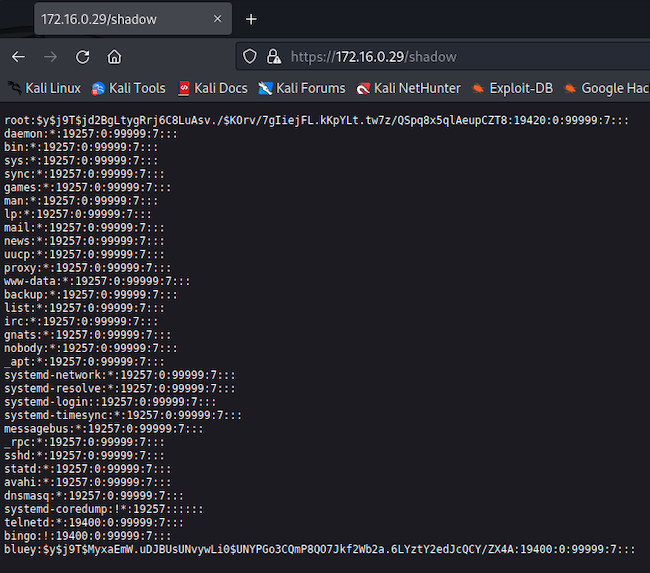
\includegraphics[width=0.8\textwidth]{img/shadow-file-433.png}
    \caption{Access to shadow file}
    \label{fig:fin8}
\end{figure}


\subsection{Evaluation of Results}
\begin{center}
    \begin{tabular}{cccc}
    \textbf{Effort to Fix:} & &\ \textbf{\textcolor{green!50!blue}{Low}}\
    \end{tabular}
\end{center}
Fix the file which sets the filename that should be opened. This should prevent the Webserver from opening files which are not intended to be opened. Also whitelisting the allowed paths could be a solution to prevent path traversal.
